\section{Struktura danych \textsc{CDLMW BP(s)}}
\label{sec:cdlmw-bp}
Struktura ta działa przy założeniu standardowego modelu obliczeń \textsc{RAM} z słowem maszynowym $w \in \Omega(\log n)$ oraz wymaga, aby częstotliwość dominanty była nie większa niż $s$.
Struktura \textsc{CDLMW BIT-PACKING}, w skrócie \textsc{CDLMW BP} (algorytm 2 z pracy \cite{chan14}) jest modyfikacją struktury \textsc{CDLMW}, która zmienia reprezentację tablicy $S$, aby była bardziej zwięzła. Ponadto nie będziemy przechowywać tablicy $S'$. Dzięki tym modyfikacjom uzyskuje mniejsze zużycie pamięci względem rozmiaru bloku, co pozwoli nam na dobranie większej liczby bloków $s=\sqrt{nw}$. Analogicznie do struktury \textsc{KMS(s)} będziemy dzielić tablicę $A$ na $s$ bloków, każdy, prócz ostatniego, o rozmiarze $t=\cl{n/s}$. $i$-ty blok $B_i$ dla $i=0,1,\dots,s-1$ reprezentuje przedział $A[it+1, \min(n,(i+1)t)]$. Struktura \textsc{CDLMW BP} wspiera następujące operacje:
\begin{enumerate}[nosep]
    \item \textsc{bcount}$(b_i,b_j)$ -- Oblicza dominantę wraz z częstotliwością przedziału $A[b_it+1: \min(n,(b_j+1)t)]$ w czasie $\Oh(n/s)$, przy założeniu $b_i \le b_j < s$.
    \item \textsc{count}$(h,i,j)$ -- Oblicza $F^A_{A[i]}(i, j)$ w czasie $\Oh(F^A_{A[i]}(i, j) - h)$. Zakładamy, że $1 \le h \le F^A_{A[i]}(i,j).$
    \item \textsc{query}$(i, j)$ -- Oblicza dominantę i jej częstotliwość w czasie $\Oh(n/s)$.
\end{enumerate}
Operacja $\textsc{bcount}(b_i, b_j)$ oblicza dokładnie to samo co było przechowywane w wartościach tablic $S[b_i, b_j]$ oraz $S'[b_i, b_j]$ w strukturze $\textsc{KMS}(s)$.

%=========================================================
\subsection{Konstrukcja}
Konstruujemy tablicę $R$ która jest opisana przy strukturze danych \textsc{CDLMW} oraz konstruujemy $\dt$ tablic $Q_x$ które są opisane przy strukturze danych \textsc{KMS}. Tworzymy, dla każdego $i \in \{0, 1, \dots, s-1\}$ ciąg binarny $T[i]$, który odpowiada wierszowi $S[i, *]$ z tablicy w algorytmie \textsc{KMS}. Dla każdego $j \in \{i, i+1, \dots, s-1\}$ dopisujemy na koniec ciągu $T[i]$ najpierw $S[i,j] - S[i, j-1]$ zer, a potem jedną jedynkę. Przyjmujemy $S[i,i-1] = 0$. Dla przykładu wiersz $2,3,5,5$ zamieniamy na ciąg binarny $001010011$.

%=========================================================
\subsection{Operacje \textsc{RANK} i \textsc{SELECT}}
Dla ciągu binarnego $B=(b_0,b_1,...,b_{k-1})$, oraz liczby $b \in \{0, 1\}$ definiujemy operację $\textsc{rank}_b(B,i) = |\{j\ |\ b_j=b \land j \in \{0, 1, \dots, i-1\}\}|$, innymi słowy $\textsc{rank}_b(B,i)$ to liczba elementów ciągu $B$ równa $b$ na przedziale $[0, i)$. Definiujemy również operację $\textsc{select}_b(B, i) = \min\{k \in \{1, 2, \dots n\}\ | \ rank_b(k)=i\}$ -- jest to indeks $i$-tego wystąpienia liczby $b$ w ciągu $B$, gdzie $i > 0$. Operacje te pozwolą nam efektywnie wyciągać informacje z ciągów binarnych zawartych w $T$. Dla przykładu, znając pozycję $p_j$ $j$-tej jedynki w binarnym ciągu $T[i]$, możemy obliczyć częstotliwość dominanty $B_i \cup B_{i+1} \dots \cup B_{i+j-1}$ poprzez zapytanie $\textsc{rank}_0(T[i],p_j)$. Oczywiście $p_j$ możemy obliczyć za pomocą zapytania $\textsc{select}_1(T[i], j)$. Dla działania algorytmu kluczowym jest, aby operacje te zużywały maksymalnie liniową liczbę bitów od długości ciągu na którym operują. \textsc{RANK} oraz \textsc{SELECT} są podstawą zwięzłych struktur danych (ang. succinct data structures), w związku z czym są dobrze zbadane (\cite{jaco89}, \cite{clar97}, \cite{rama07}). Dla obu operacji istnieją struktury zużywające podliniową pamięć i pozwalające na zapytania w stałym czasie, przy liniowym czasie konstrukcji. My jednak zdecydowaliśmy się zaimplementować bardziej praktyczne (\cite{vign08}, \cite{nakp09}) wersje tych operacji, które zużywają większą, liniową pamięć. Opiszemy implementację tych operacji w późniejszej sekcji.

%=========================================================
\subsection{Operacja \textsc{bcount}}
\begin{algorithm}
    \caption{Operacja \textsc{bcount}}
    \label{alg:cdlmw-bp-bcount}
    \begin{algorithmic}[1]
        \Function{bcount}{$b_i$,$b_j$}
            \State $pos_{b_j} \gets select_1(T[b_i], b_j-b_i+1)$
            \State $freq \gets rank_0(T[b_i], pos_{b_j})$
            \State $pos_{last} \gets select_0(T[b_i], freq)$
            \State $b_{last} \gets rank_1(T[b_i], pos_{last}) + b_i$
            \State $first \gets tb_{last}+1$
            \State $last \gets \min(n,first+t)$
            \For{$k \gets first, \dots, last$}
                \If {$R[k]-freq+1 \ge 0 \land Q_{A[k]}[R[k]-freq+1] \ge first$}
                    \State \Return $freq, A[k]$
                \EndIf
            \EndFor
        \EndFunction
    \end{algorithmic}
\end{algorithm}
Załóżmy, że chcemy obliczyć dominantę $B_{b_i,b_j} = B_{b_i} \cup B_{b_i+1} \cup \dots \cup B_{b_j}$ oraz jej częstotliwość. Oznaczmy przez $l=b_it+1$, $r=(b_j+1)t$ odpowiednio lewy oraz prawy koniec $B_{b_i,b_j}$.
Z konstrukcji $T[b_i]$ łatwo zauważyć, że częstotliwość dominanty $B_{b_i,b_j}$ to liczba zer między początkiem ciągu $T[b_i]$, a jego $(b_j-b_i+1)$-tą jedynką. Robimy to w linijkach 2-3. Następnie zauważmy, że ostatnie zero występujące przed $(b_j-b_i+1)$-tą jedynką zostało wygenerowane przez pewną dominantę $B_{b_i, b_j}$. Możemy znaleźć pozycję tego zera jednym zapytaniem $\textsc{select}_0$, robimy to w 4-tej linijce. Znając pozycję ostatniego zera wygenerowanego przez dominantę $B_{b_i,b_j}$ łatwo znaleźć, w którym bloku ta dominanta się znajduje za pomocą operacji $\textsc{select}_1$. Znajdujemy dominantę $B_{b_i, b_j}$ skanując ostatni blok w którym się ona zawiera, dla każdego elementu bloku sprawdzamy czy występuje on co najmniej $F^A(l, r)$ razy w $B_{b_i,b_j}$.

%=========================================================
\subsection{Operacje \textsc{count} oraz \textsc{query}}
Operacja \textsc{count} pozostaje niezmieniona względem struktury \textsc{CDLMW(s)}, a jedyną zmianą w operacji \textsc{query} jest sposób obliczania dominanty $B_{b_i+1, b_j-1}$. Używamy do tego operacji \textsc{bcount} zamiast dostępu do tablic $S$, $S'$.

%=========================================================
\subsection{Analiza złożoności czasowej}
\paragraph{Konstrukcja} Jedyna zmiana analizy względem struktury \textsc{CDLMW(s)} jest konstrukcja binarnych ciągów $T[i]$. Ciągi te konstruujemy skanując tablicę $A$ $s$ razy. Inicjalizacja operacji \textsc{rank} oraz \textsc{select} jest liniowa od długości ciągu binarnego. Ponieważ założyliśmy, że częstotliwość dominanty jest ograniczona przez $s$ każdy ciąg binarny jest maksymalnie rozmiaru $2s$.
Konstrukcja $T$ wraz z \textsc{rank} i \textsc{select} zajmuje $\Oh(ns)$ czasu. Łącznie na konstrukcje potrzebujemy $\Oh(ns)$ czasu.
\paragraph{Operajca \textsc{bcount}} Używamy po 2 operacje \textsc{rank} i \textsc{select}, które zajmują stały czas. Ponadto liniowo skanujemy jeden blok o rozmiarze $t$. Łącznie potrzebujemy $O(t)$ czasu.
\paragraph{Operacje \textsc{count}} Nic nie zostało zmienione względem poprzedniej struktury danych. $\Oh(F^A_{A[i]}(i, j) - h)$ czasu.
\paragraph{Operacja \textsc{query}} Względem poprzedniej struktury danych obliczenie zmiennych $mfreq$ oraz $mmode$ wzrosło do $\Oh(t)$ ponieważ używamy operacji \textsc{bcount}. Jednakże nie zmienia to łącznej złożoności czasowej $\Oh(t)$.

%=========================================================
\subsection{Analiza złożoności pamięciowej}
\paragraph{Konstrukcja} Ponieważ założyliśmy model \textsc{RAM} możemy ciągi binarne $T$ spakować w słowa maszynowe dzięki czemu mamy $s$ ciągów, każdy zajmujący $\Oh(s/w)$ słów maszynowych. Zatem łącznie na ciągi $T$ potrzebujemy $\Oh(s^2/w)$ słów maszynowych, wliczając w to wsparcie dla operacji $\textsc{rank}$ oraz $\textsc{select}$. Doliczając do tego tablicę $R$ oraz $\dt$ tablic $Q_x$ łącznie struktura danych zużywa $\Oh(n + s^2/w)$ pamięci.
\paragraph{Operajca \textsc{bcount}} Używamy stałej pamięci podczas tej operacji.
\paragraph{Operacje \textsc{count} i \textsc{query}} Koszt pamięci tych operacji pozostaje w dalszym ciągu stały.

%=========================================================
\subsection{Dobór parametru s}
Dzięki zmniejszonemu zużyciu pamięci możemy dobrać większą liczbę bloków $s=\sqrt{nw}$ co da nam strukturę o liniowej pamięci, która pozwala obliczać dominanty na dowolnym przedziale w czasie $\Oh(\sqrt{n/w})$.

%=========================================================
\subsection{Implementacja}
W sekcji tej będziemy operować na binarnym ciągu $B=(b_0, b_1, \dots, b_{k-1})$. Dla którego będziemy chcieli szybko odpowiadać na zapytania $\textsc{rank}$ oraz $\textsc{select}$.
\subsubsection{\textsc{rank}}
\begin{figure}[H]
    \centering
    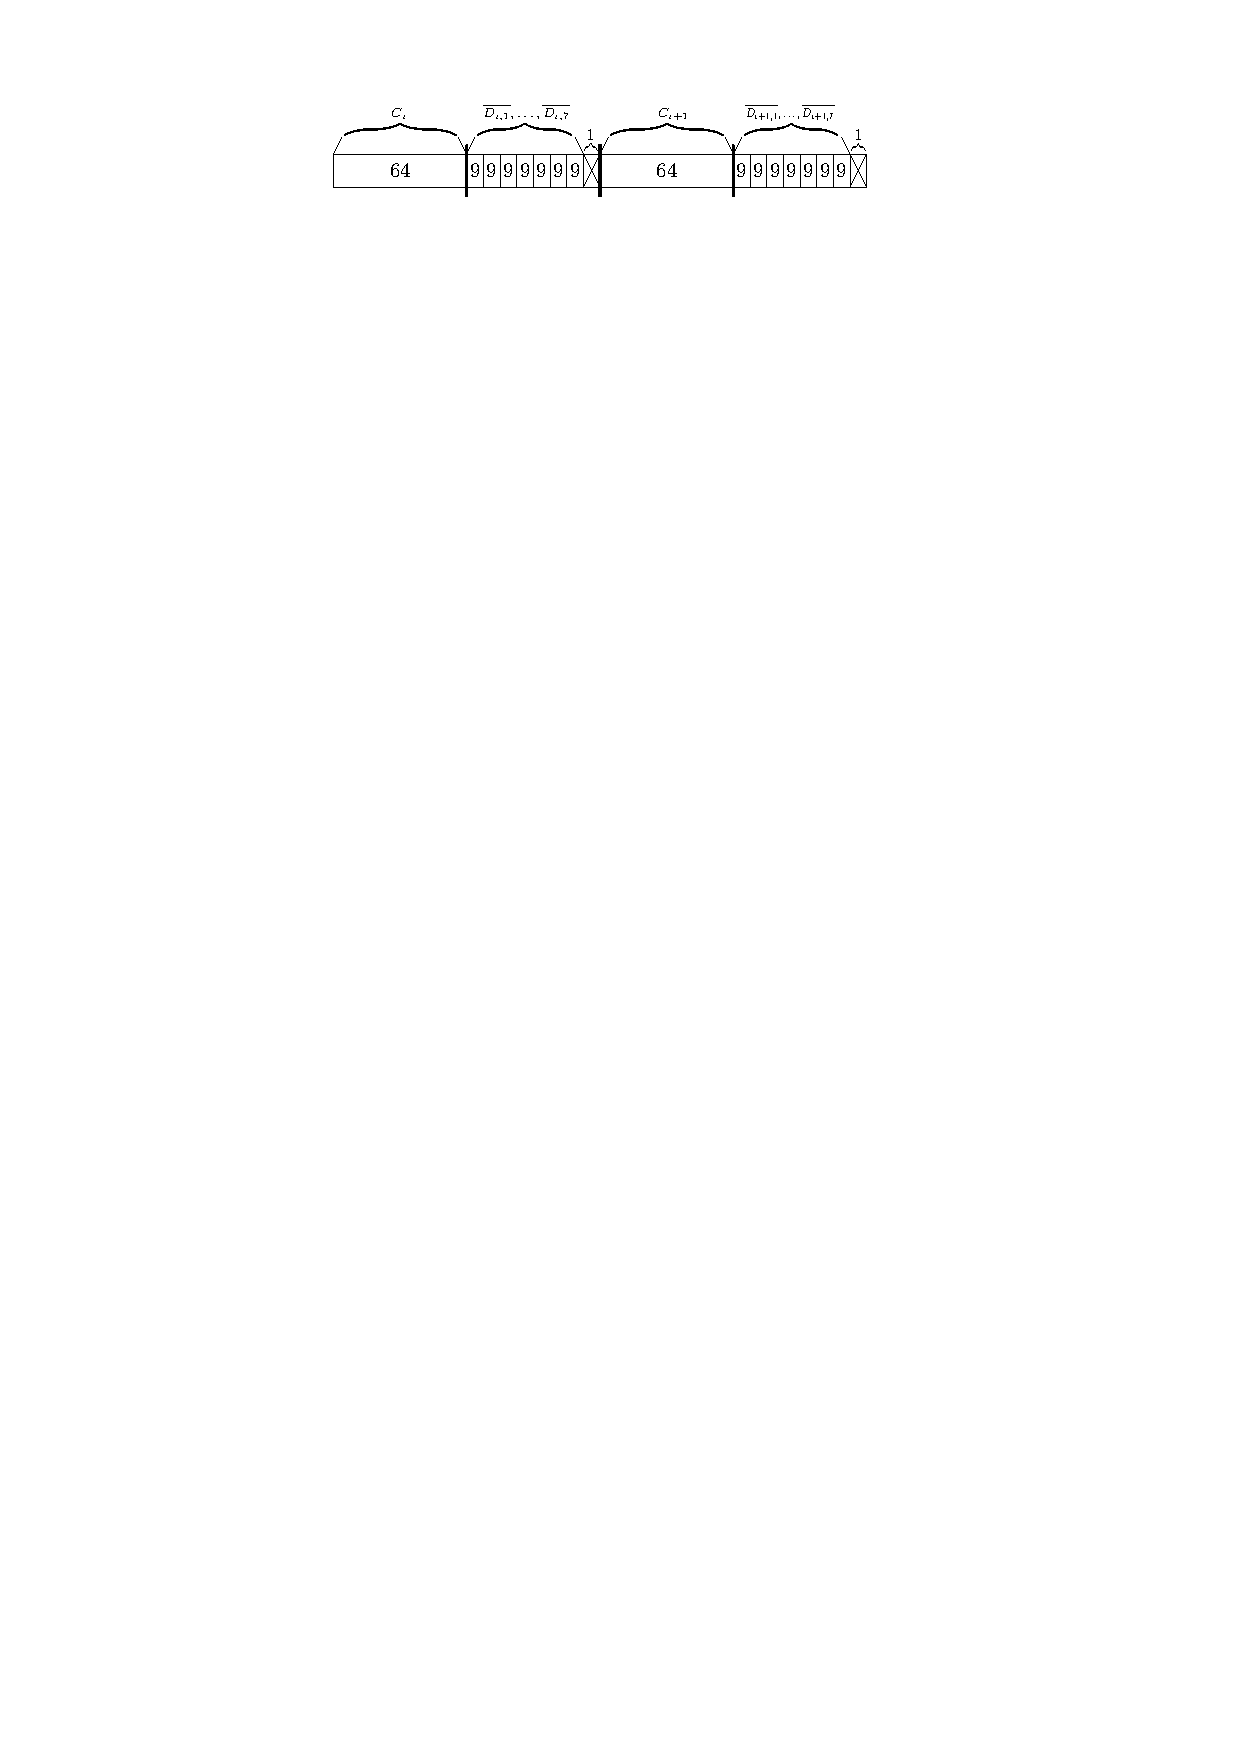
\includegraphics[scale=1.2]{images/rank9-mem-layout.pdf}
    \caption{Fragment układu pamięci danych $\overline{C_i}, \overline{C_{i+1}}, \overline{D_{i,*}}, \overline{D_{i+1,*}}$}. Liczby reprezentują rozmiar danych w bitach.
    \label{fig:rank9-mem}
\end{figure}
Zaimplementowaliśmy strukturę $\textsc{RANK9}$ z pracy \cite{vign08} autorstwa Sebastiano Vigna, która pozwala odpowiadać na zapytania $\textsc{rank}_1$. Struktura ta jest specjalnie zoptymalizowana pod procesory o $64$-bitowym słowie maszynowym.
\paragraph{Konstrukcja}
Dla uproszczenia załóżmy, że $k$ jest wielokrotnością $512$. Dzielimy ciąg $B$ na $k/512$ bloków $C_0, C_2, \dots, C_{k/512-1}$, gdzie $i$-ty blok reprezentuje bity $B[512i:512(i+1)-1]$. Ponadto, każdy blok $C_i$ dzielimy na 8 podbloków $D_{i,0}, \dots, D_{i,7}$, gdzie $j$-ty podblok reprezentuje bity $B[512i+64j: 512i+64(j+1)-1]$. Dla każdego bloku $C_i$ przechowujemy w liczbie $64$-bitowej $\overline{C_i}=\textsc{rank}_1(B, 512i)$. Ponadto dla każdego podbloku $D_{i,j}$ zapisujemy używając $9$-bitów $\overline{D_{i,j}}=\textsc{rank}_1(C_i, 64j)$ -- możemy to zrobić ponieważ, każdy podblok przechowuje $\textsc{rank}_1$ ciągu o rozmiarze co najwyżej 512 bitów zatem wynik zmieści się w $9$ bitach.
\paragraph{Zapytanie}
Oznaczmy przez $C_i, D_{i,j}$ blok i podblok do którego należy $B[l-1]$. Obliczamy zapytanie $\textsc{rank}_1(B,l)$ następująco: $\overline{C_i} + \overline{D_{i,j}} + \textsc{rank}_1(B[512i+64j:i], l-512i-64j)$. Ostatni $\textsc{rank}_1$ jest nad ciągiem o maksymalnej długości $64$, który możemy obsłużyć za pomocą instrukcji \lstinline{_mm_countbits_64}\footnote{\url{https://software.intel.com/sites/landingpage/IntrinsicsGuide/\#text=_mm_countbits_64}} w czasie stałym. W praktyce jednak, używamy funkcji wbudowanej \lstinline{__builtin_popcountll}\footnote{\url{https://gcc.gnu.org/onlinedocs/gcc/Other-Builtins.html}}, która jest wspierana przez większość dużych kompilatorów języka c++ (GCC, Clang, MSVC). Generuje ona odpowiedni kod maszynowy w zależności od docelowej platformy.

\paragraph{Optymalizacje}
 $\overline{D_{i,0}}$ zawsze wynosi 0, zatem nie musimy przechowywać wartości tej w pamięci. Dla każdego bloku $C_i$ przechowujemy $\overline{C_i}$ oraz $\overline{D_{i,j}}$, gdzie $j=1\dots7$. $\overline{C_i}$ zajmuje $64$ bity, a $\overline{D_{i,j}}$ łącznie zużywają $7*9=63$ bity, więc możemy wszystkie $\overline{D_{i,j}}$ spakować do jednego słowa maszynowego. Ponadto zauważamy, że zaraz po odczycie $\overline{C_i}$ robimy odczyt $\overline{D_{i,j}}$ zatem pakujemy te 2 słowa maszynowe obok siebie w pamięci, w celu zminimalizowania liczby nietrafień w pamięć podręczną procesora. Można zobaczyć jak wygląda układ pamięci tych danych na rysunku \ref{fig:rank9-mem}. Dla każdych $512$-bitów używamy 2 $64$-bitowe słowa maszynowe. Podsumowując narzut pamięciowy operacji $\textsc{rank}_1$ wynosi $128\cl{k/512} \approx 0.25k$ bitów.

\paragraph{$\textsc{rank}_0$} $\textsc{rank}_0(B, i)$ możemy obsługiwać poprzez prostą obserwacje: $\textsc{rank}_0(B, i) = i - \textsc{rank}_1(B, i)$.

\subsubsection{\textsc{select}}
\begin{figure}[H]
    \centering
    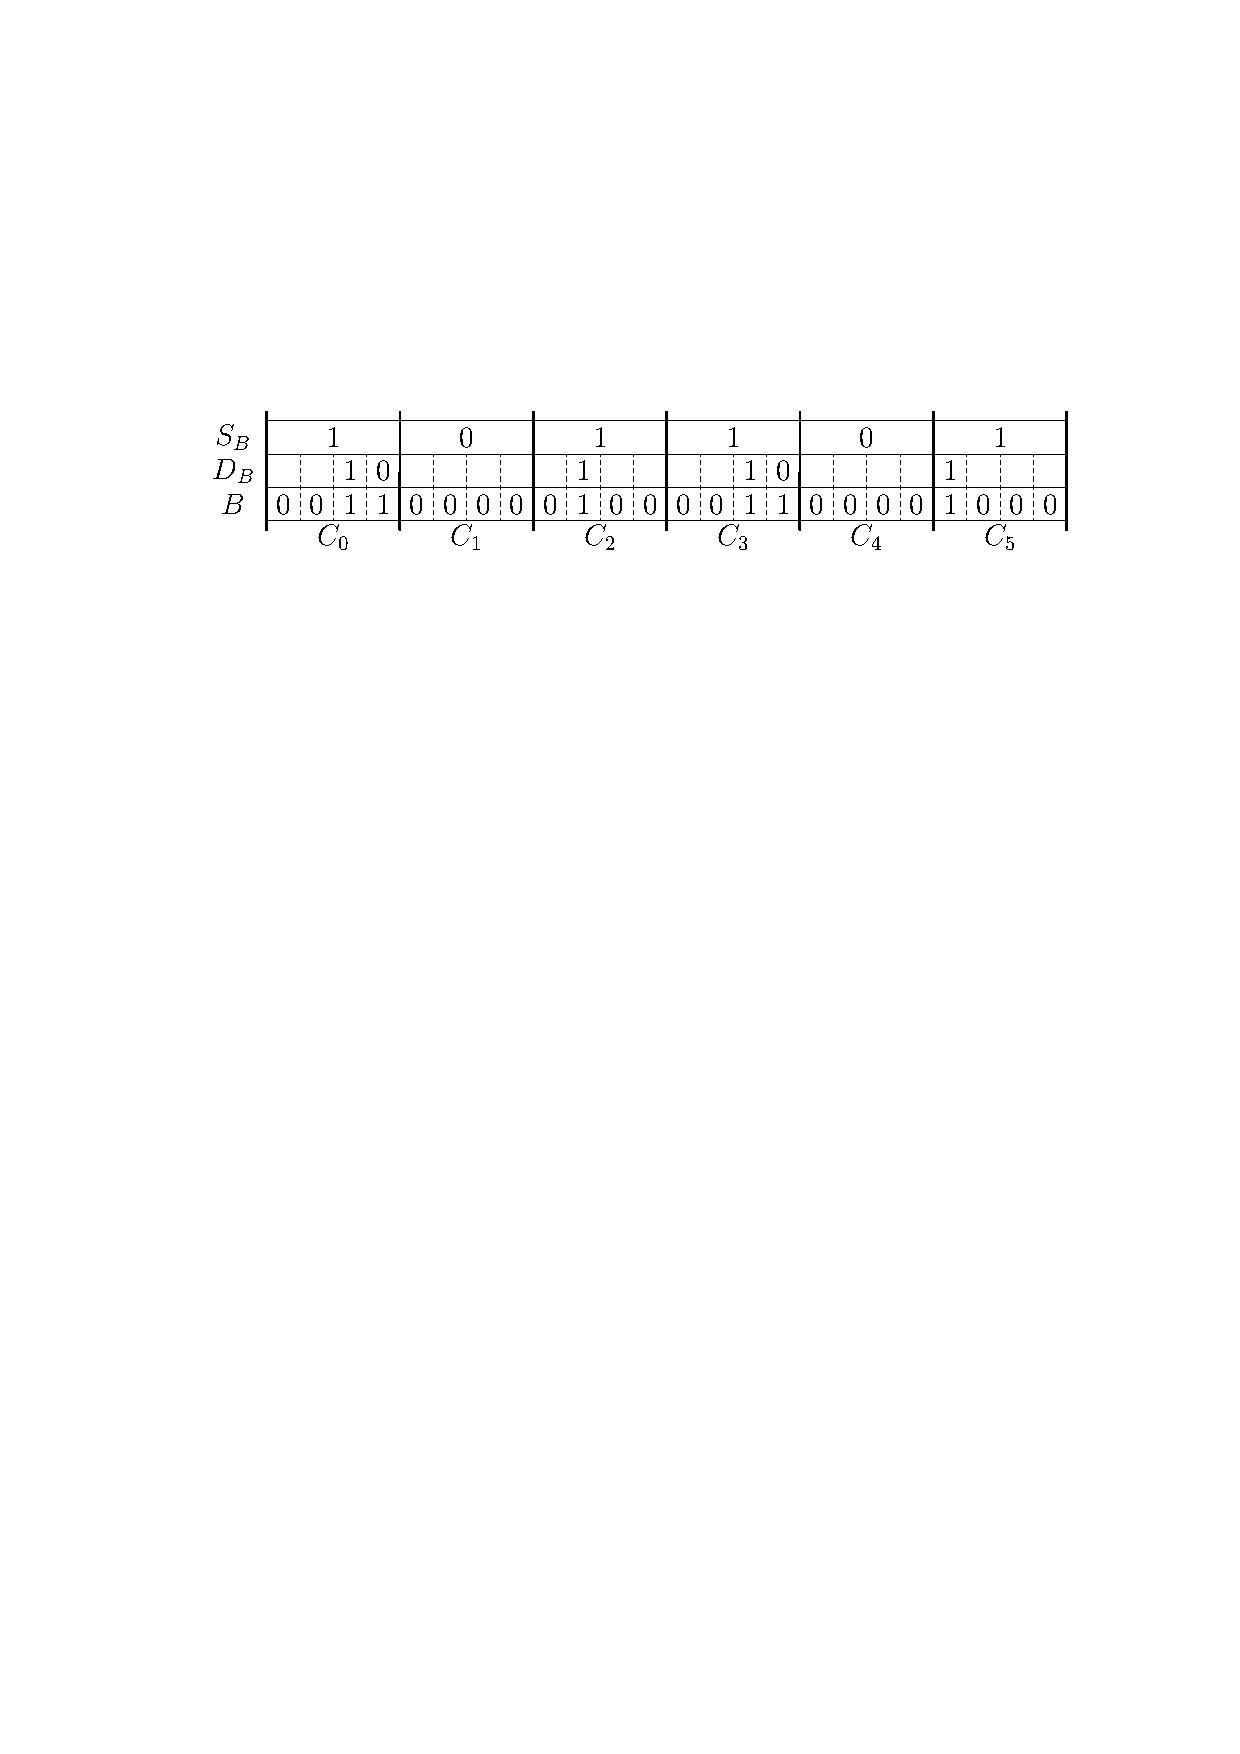
\includegraphics[scale=0.8]{images/select.pdf}
    \caption{Przykładowy ciąg $B$ oraz jego ciąg streszczony $S_B$ oraz ciąg przerywający $D_B$ z zaznaczonymi blokami $C_0,\dots,C_5$. Długość słowa maszynowego na tym przykładzie wynosi $w=4$.}
    % \caption{Fragment układu pamięci danych $\overline{C_i}, \overline{C_{i+1}}, \overline{D_{i,*}}, \overline{D_{i+1,*}}$}. Liczby reprezentują rozmiar danych w bitach.
    \label{fig:select}
\end{figure}\vspace{-0.5em}
Zaimplementowaliśmy lekko zmodyfikowany algorytm 2 z pracy \cite{nakp09} autorstwa Chae i innych. Nasza modyfikacja polega na wykorzystaniu dwóch instrukcji \lstinline{_pdep_u64}\footnote{\url{https://software.intel.com/sites/landingpage/IntrinsicsGuide/\#text=_pdep_u64}},
\lstinline{_mm_tzcnt_64}\footnote{\url{https://software.intel.com/sites/landingpage/IntrinsicsGuide/\#text=_mm_tzcnt_64}} dostępnych na procesorach Intel oraz AMD. Instrukcje te pozwolą nam na wykonanie operacji $\textsc{select}_1$ wewnątrz słowa maszynowego w stałym czasie i stałej pamięci.
Oznaczamy przez $m$ liczbę jedynek w ciągu $B$. Dla uproszczenia załóżmy, że $k$ jest wielokrotnością $w$. Dzielimy ciąg $B$ na $k/w$ bloków $C_0, C_1, \dots, C_{k/w-1}$, gdzie $i$-ty blok reprezentuje bity $B[wi:w(i+1)-1]$. 

Dla ciągu binarnego $B$ definiujemy 2 pochodne ciągi binarne:
\begin{enumerate}[nosep]
    \item \emph{Streszczony ciąg} $S_B[0:k/w-1]$ ciągu $B$ ma na $i$-tej pozycji $1$ gdy, dowolny bit bloku $C_i$ jest nie zerowy. W przeciwnym wypadku $S_B[i] = 0$.
    \item \emph{Przerywający ciąg} $D_B[0:m-1]$ ciągu $B$ ma na $i$-tej pozycji $1$ gdy $(i+1)$-wsza jedynka ciągu $B$ jest pierwszą jedynką w bloku ją zawierającym. W przeciwnym przypadku $D_B[i]=0$.
\end{enumerate}
\vspace{-0.5em}\paragraph{Redukcja do $\textsc{select}_1$ w pojedynczym bloku}
Naszym celem będzie zredukowanie $\textsc{select}_1(B, i)$ do operacji $\textsc{select}_1$ wewnątrz pojedynczego bloku. Aby to osiągnąć najpierw pokażemy jak obliczyć $\textsc{select}_1(S_B, i)$. Ciąg $S_B$ jest krótki, jego rozmiar wynosi $n/w$. Pozwala to nam na zapamiętanie pozycji wszystkich jedynek. Potrzebujemy $\log(n/w)$ bitów, aby zapisać jeden indeks. Indeksów do zapisania jest co najwyżej $n/w$. Korzystając z założenia, że $w \in \Omega(\log n)$ możemy oszacować potrzebną pamięć przez $\Oh(n/\log(n) \log(n/\log(n))) \subset \Oh(n/\log(n) \log(n)) = \Oh(n)$. Dzięki operacji $\textsc{select}_1$ dla ciągu $S_B$ jesteśmy wstanie znaleźć indeks $k$-tego niepustego bloku w czasie stałym. Ponadto możemy znaleźć numer niepustego bloku w którym znajduje się $i$-ta jedynka za pomocą operacji $\textsc{rank}_1(D_B, i)$. Przy użyciu tych dwóch operacji potrafimy znaleźć indeks $s_i$ bloku w którym jest $i$-ta jedynka oraz $p=\textsc{rank}_1(B, s_iw)$ liczbę jedynek poprzedzającą blok $C_{s_i}$. Łącząc to wszystko dostajemy wzór: $\textsc{select}_1(B, i) = s_iw + \textsc{select}_1(C_{s_i}, i-p)$. Zredukowaliśmy $\textsc{select}_1(B, i)$ do $\textsc{select}_1$ w bloku $C_{s_i}$. Dla przykładu znajdziemy 5-tą jedynkę w ciągu $B$ na rysunku \ref{fig:select}. Najpierw znajdujemy numer niepustego bloku w którym znajduje się 5-ta jedynka $\textsc{rank}_1(D_B,5) = 3$. Następnie obliczamy indeks bloku $s_i$ w którym znajduje się 5-ta jedynka $s_i = \textsc{select}_1(S_B, 3) = 3$. Następnie liczymy $p$ liczbę jedynek poprzedzającą blok $s_i$: $p=\textsc{rank}_1(B, s_iw) = \textsc{rank}_1(B, 12) = 3$. Korzystamy ze wzoru $\textsc{select}_1(B, 5) = s_iw + \textsc{select}_1(C_{3}, 2) = 12+3 = 15$. Jak obliczyć $\textsc{select}_1$ w bloku $C_{3}$ pokazujemy w następnym paragrafie. 
\vspace{-0.5em}\paragraph{$\textsc{select}_1$ w pojedynczym bloku}W tym przypadku używamy dwóch instrukcji procesora \lstinline{_pdep_u64} oraz \lstinline{_mm_tzcnt_64}. Niech $a[0:63], msk[0:63]$ to $64$-bitowe liczby. Oznaczmy przez $l$ liczbę niezerowych bitów $msk$ oraz $x_0, \dots, x_{l-1}$ indeksy tych bitów. Wówczas \lstinline{_pdep_u64}$(a, msk)$ zwróci $64$-bitową liczbę $K[0:63]$ zdefiniowaną jako $K[x_i] = a[i]$ oraz $K[j] = 0$ dla $j \ne x_i$. W szczególności \lstinline{_pdep_u64}$(2^{c-1}, x)$ zwróci liczbę, która ma jeden nie zerowy bit na pozycji $c$-tej jedynki liczby $x$. Instrukcja \lstinline{_mm_tzcnt_64} umożliwia nam znalezienie tej pozycji poprzez zliczenie końcowych zer. Dla przykładu znajdziemy $5$-tą jedynkę liczby $a=010011001101_{2}$. \lstinline{_pdep_u64}$(2^{5-1}=00001_{2}, 010011001101_{2}) = 000000000100_{2}$. Teraz liczmy końcowe zera -- \lstinline{_mm_tzcnt_64}$(000000000100_{2})$ = 9. $5$-ta jedynka liczby a znajduje się na $9$-tej pozycji.

\vspace{-0.5em}\paragraph{Narzut pamięciowy} Potrzebujemy wykonywać operacje \textsc{rank} dla ciągów $B$ oraz $D_B$, zakładając użycie struktury \textsc{rank9} potrzebujemy $\approx 2*0.25k = 0.5k$ bitów. Sam ciąg $D_B$ zajmuje pesymistycznie $k$ bitów. Ponadto, użyliśmy $\textsc{select}_1$ na ciągu $S_B$, dla którego zapisaliśmy wszystkie pozycje jedynek. Zakładając $w \ge \log k$ zużywamy co najwyżej $k$ bitów. Łącznie potrzebujemy co najwyżej $2.5k$ bitów.
\newpage